\chapter{Future colliders}
The chapter begins with a short description of the most important goals in today's particle physics, starting from the possibilities opened by the discovery of the Higgs boson.\\
It continues with an overview on the different projects among high-energy $e^+e^-$ colliders, both circular and linear (also known as ``electroweak factories").\\
Eventually, the IDEA Detector concept is described as a general-purpose detector designed for future $e^+e^-$ circular colliders.

\section{Physics goals}
With the discovery of the Higgs boson ($H$) in 2012 by the ATLAS and CMS Collaborations \cite{ATLAS_H, CMS_H}, a new era has been opened where the new boson is not only a research object but also a tool for new particle physics studies.\\

Thanks to the relatively small mass, $\simeq 125$ GeV, the Higgs boson production is within the reach of high-luminosity future circular colliders. Their main production mechanism is the so-called Higgs-strahlung process, in which the Higgs recoils over a $Z$-boson produced at $E_{cm}\simeq 240$ GeV ($e^+ e^- \rightarrow Z H$).
In $HZ$ events, the recoil mass (defined as the invariant mass of the system recoiling against the Z boson) peaks at the Higgs mass, thus allowing to tag the events independently of the $H$ decay mode.
This process allows to measure the Higgs production cross section in a model-independent way. The other couplings are eventually extracted through branching-ratio and width measurements with a subpercent precision.

%The total Higgs production cross section can be measured in the Higgstrahlung process  looking at its presence as the recoil to the $Z$. In this way the $H$ boson is directly coupled to the $Z$ measurement.
%The $H Z$ events have their recoil mass equal to $m_H$, hence Higgs bosons can be counted from the accumulation around the $H$ mass value, allowing to determine the $H Z$ cross section ($\sigma_{HZ}$).
%In particular, the total cross section could be determined independently of the $H$ decay, by counting the Higgsstrahlung events characterised by a leptonic decay: $Z \rightarrow l^+ l^-$.
%This method disentangled the $H$ production from its decay, providing a model-independent determination of its total width and its other couplings through branching ratio measurements with a sub-percent precision.\\

The $H$ couplings to the first Standard Model family particles (i.e. electron, quark up and quark down), because of their small masses and related decay branching ratios, will not be directly measurable at these colliders. 
However, with beam energies $\simeq 125.09$ GeV, corresponding to the $H$ pole mass, leptonic colliders can contribute to set upper limits to the electron Yukawa coupling by taking advantage from the resonant $H$ production.
Also the $t$ Yukawa coupling and the $H$ self-coupling will not be directly measurable because their masses are too large for a kinematically open decay.
However, the CERN future electron-positron circular collider (FCC-ee), operating at $\sqrt{s} = 350$ GeV, could measure the $t$ Yukawa coupling with a precision of $10\%$ thanks to higher order corrections of processes at the $t\Bar{t}$ threshold.\\

%It is possible to predict mass and properties of the top-quark and of the bosons $Z$, $W$ and $H$ using the Standard Model. This predictions are obtained from precise measurements in the Electroweak sector and theoretical calculations.
%Quantities called Electroweak Precision Observables (EWPOs) can establish the presence of new physics. For this reason EWPOs measurements represent another important component in the future colliders physics program.
%The future leptonic colliders has the purpose to significantly improve in the precision (more than an order of magnitude actual one) their value and provide a broad set of EWPOs, giving access to many possible new physics sources.
%Therefore, the main  studies will concern the $Z$ pole, the light neutrino species number and the $W^+W^-$ and $t\Bar{t}$ thresholds.

\section{Leptonic colliders}\label{sec:Coll-ee}
Precise measurements of Higgs boson properties, together with those of the $Z$ and $W$ bosons, will provide important tests of the SM fundamental physics principles and will be essential for Beyond-the-Standard-Model (BSM) physics studies.
At present, the landscape of high energy physics includes four different electroweak-factory proposals:
\begin{itemize}
    \item the \textit{Future Circular Collider $e^+e^-$} (FCC-ee), at CERN;
    \item the \textit{Circular Electron Positron Collider} (CEPC), in China;
    \item the \textit{International Linear Collider} (ILC), in Japan;
    \item the \textit{Compact LInear Collider} (CLIC), at CERN.
\end{itemize}
Fig \ref{fig:roadmap} shows the possible timeline envisaged for the main future collider projects.
In the following sections, a brief description of each one of them will be provided.

\begin{sidewaysfigure}
	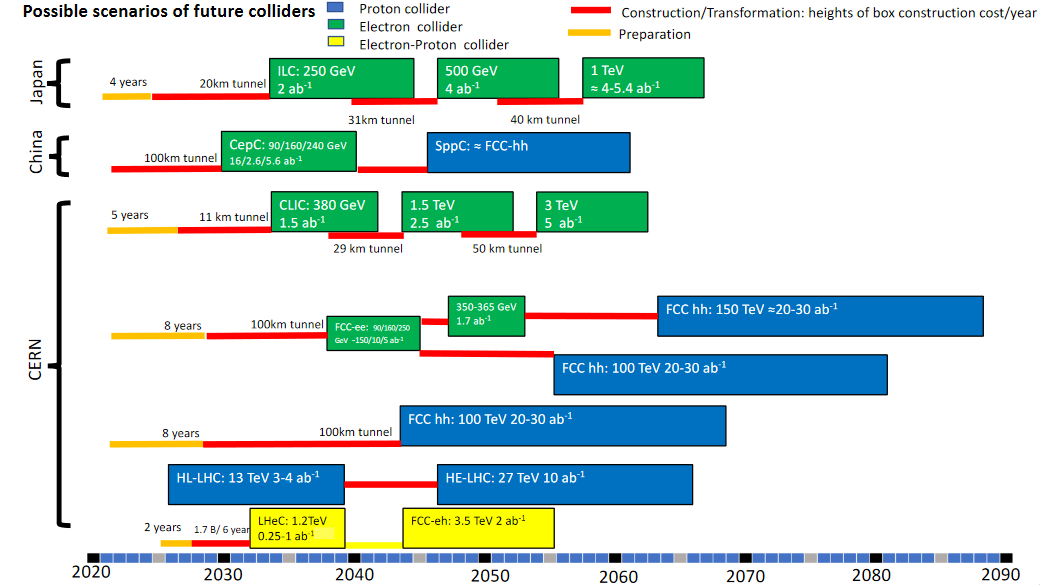
\includegraphics[width = 0.95\textwidth]{IMG/Cap1/Roadmap.png}
	\caption{Possible  timelines  of  future  colliders.  It includes high-energy $e^+e^-$ (ILC,  CLIC,  CEPC  and  FCC-ee), $pp$ (FCC-hh  and HL-LHC) and $e-p$ (LHeC and FCC-eh) machines. Image from \cite{roadmap}.}
	\label{fig:roadmap}
\end{sidewaysfigure}

\subsection*{Future Circular Collider $e^+e^-$}
A post-LHC circular collider at CERN has been proposed with the name of Future Circular Collider (FCC) project \cite{FCC}. FCC is staged in a first lepton collider (FCC-ee) \cite{FCC-ee} phase followed by a hadron collider (FCC-hh) \cite{FCC-hh} with a final target centre-of-mass energy of $100$ TeV. A common tunnel, about $100$ km long, is designed to host both of them. With this choice the same facility could potentially house an electron-hadron collider.\\
FCC-ee is designed to provide the highest possible statistics for the $Z$, $W$ and $H$ bosons, and $t$ quarks. At present, it is supposed to operate at centre-of-mass energies ranging from $88$ to $365$ GeV in four different ($\sqrt{s}$) operating points:
\begin{itemize}
    \item $\simeq 91$ GeV, corresponding to the $Z$ pole;
    \item $\simeq 160$ GeV, corresponding to the $W^+W^-$ production threshold;
    \item $\simeq 240$ GeV, corresponding to the $ZH$ production threshold;
    \item $\simeq 340-365$ GeV, corresponding to the $t\Bar{t}$ threshold.
\end{itemize}

The FCC-ee project fits over the present CERN accelerator complex, where the injector chain makes use of a $6$ GeV linac, a damping ring and the CERN SPS as a pre-booster. The baseline layout, sketched in Figure \ref{fig:FCC-ee}, is designed with two different interaction points.\\
The task of increasing our knowledge of many of the electroweak observables by one or two orders of magnitude better than the current one sets challenging constrains to the integrated luminosities needed. These values range from $0.2$ ab$^{-1}$, for the measurement of the top-quark mass and width, to $100$ ab$^{-1}$, for the measurement of the effective weak mixing angle.
These luminosities can be achieve in a reasonable amount of time only by circular colliders (see Figure \ref{fig:FCC-ee_lum}). 

\begin{figure}
	\centering
	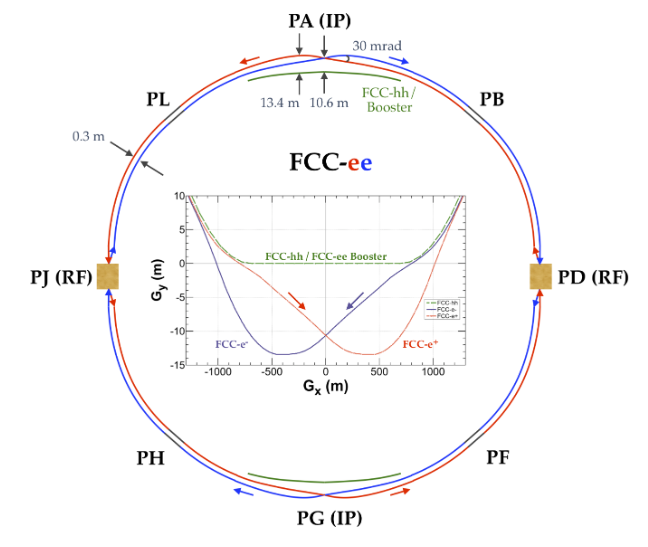
\includegraphics[width=.65\textwidth]{IMG/Cap1/FCC-ee.png}
	\caption{Schematic view of the FCC-ee. Image from \cite{FCC}.}
	\label{fig:FCC-ee}
\end{figure}

\begin{figure}
	\centering
	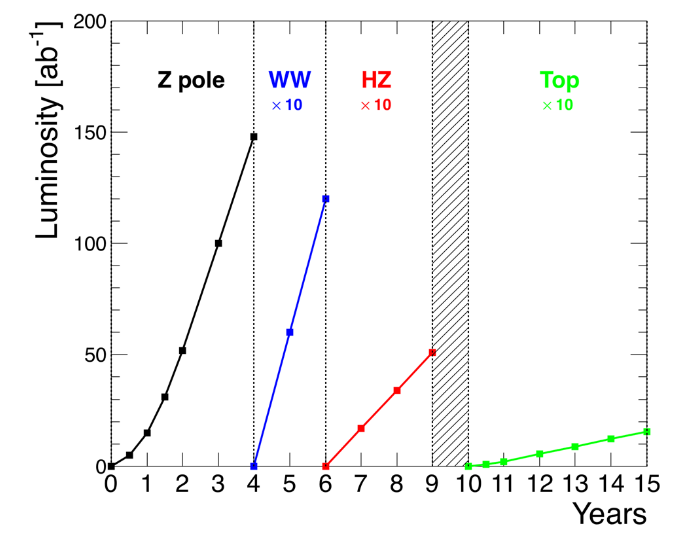
\includegraphics[width=.7\textwidth]{IMG/Cap1/FCC-ee_lum.png}
	\caption{Integrated FCC-ee luminosity during 15 years of operation. Image from \cite{FCC-ee}.}
	\label{fig:FCC-ee_lum}
\end{figure}

\subsection*{Circular Electron Positron Collider}
The Circular Electron Positron Collider (CEPC) is an international project initiated and hosted by China addressing high-luminosity $e^+e^-$ collisions. It is designed to operate at centre-of-mass energies of $240$ GeV (as an $H$ factory exploiting the $e^+e^- \rightarrow ZH$ process), $91.2$ GeV ($Z$ pole) and $160$ GeV ($W^+W^-$ threshold).\\

The present design, similarly to the FCC-ee, foresees a double ring structure, sketched in Figure \ref{fig:CEPC} with a circumference of $100$ km and two interaction points. The same $100$ km-long tunnel could also host a Super Proton-Proton Collider (SPPC) which, without removing the CEPC ring, gives the possibility to perform electron-proton collisions. As described in the conceptual design report \cite{CEPC_design1, CEPC_design2}, the main accelerator is preceded by a linear accelerator, a damping ring and a booster.\\
Associated to the three operating $\sqrt{s}$ values the instantaneous luminosities are expected to reach $3 \times 10^{34}$, $32 \times 10^{34}$ and $10 \times 10^{34}$ cm$^{-2}$s$^{-1}$, respectively.
CEPC will produce, over is planned operative time, large samples (more than one million) of Higgs, one trillion of $Z$ bosons and about 100 million of $W^+W^-$ events, allowing precise measurements of many electroweak parameters.\\

\begin{figure}
	\centering
	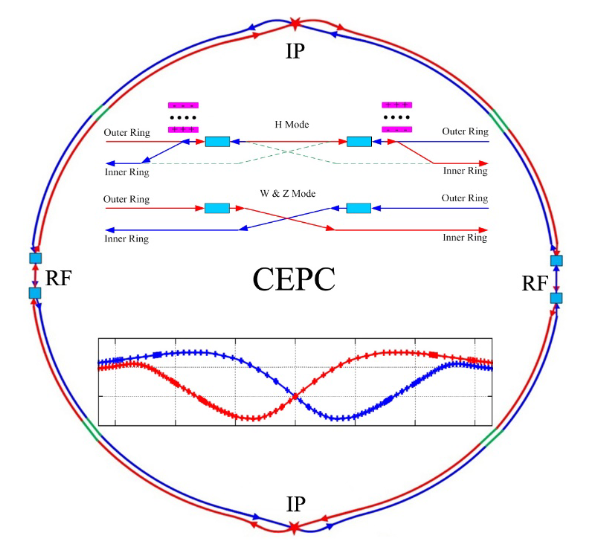
\includegraphics[width=.65\textwidth]{IMG/Cap1/CEPC.png}
	\caption{Schematic view of the CEPC. Image from \cite{CEPC_design2}.}
	\label{fig:CEPC}
\end{figure}

According to \cite{CEPC_schedule}, the CEPC construction could possibly start within few years in order to be completed by 2030, a very aggressive time schedule compared to the other collider proposals.

\subsection*{International Linear Collider}
The ILC is an $e^+e^-$ linear collider that, at the current state (ILC250), provides a $250$ GeV centre-of-mass energy.
The ILC accelerator is based on SuperConducting RadioFrequency (SCRF) cavities already in use at the European X-ray Free Electron Laser facility (E-XFEL), located at DESY/Hamburg.\\

The design luminosity is $1.35-1.5 \times 10^{34}$ cm$^{-2}$s$^{-1}$ at $E_{cm} = 250$ GeV with a corresponding integrated luminosity ranging from $400$ fb$^{-1}$ (in the first years) up to $2$ ab$^{-1}$ (after future upgrades).
The ILC250 is $20.5$ km long with two main arms, mostly occupied by the electron and positron linacs, at a $14$ mrad crossing angle. The ILC candidate site is in the Kitakami region in northern Japan. A sketch of the ILC250 is shown in Figure \ref{fig:ILC250}.\\
In its current state, the SCRF cavities will reach frequency values of $1.3$ GHz providing a gradient of $31.5-35$ MV$/$m while operating in a cryogenic infrastructure at $2$ K.\\

The first stage of ILC has the task to measure the $H$ parameters and its model-independent determination by studying the $e^+e^- \rightarrow ZH$ collisions at $\sqrt{s}= 250$ GeV.
Two energy upgrades are currently foreseen for extending the centre-of-mass energy to $500$ GeV and $1$ TeV.
The main goals for the higher-energy physics runs cover improved precision measurements of the top-quark mass, the top-quark electroweak couplings, the Higgs coupling to the top quark, and the triple-Higgs coupling \cite{ILC_global_project}.\\

\begin{figure}
	\centering
	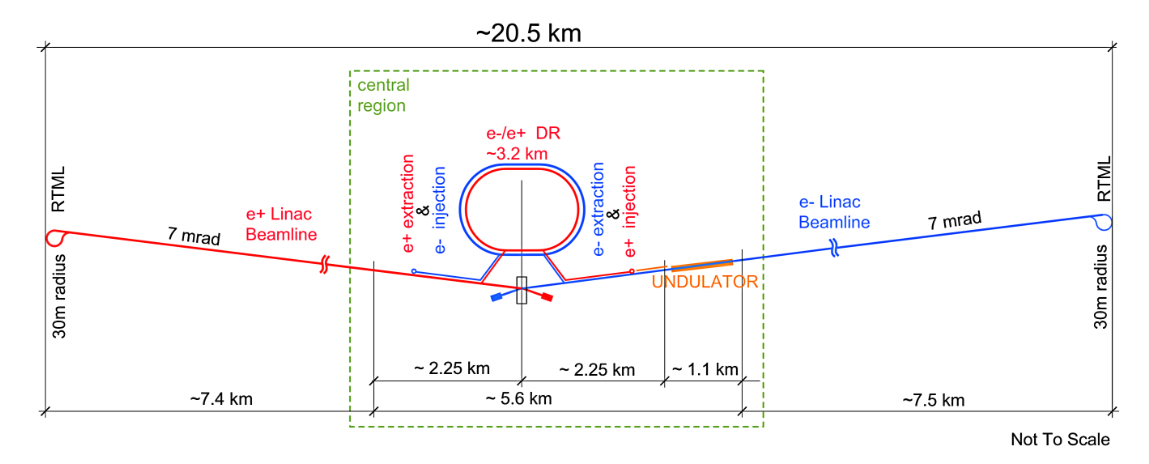
\includegraphics[width=.8\textwidth]{IMG/Cap1/ILC.png}
	\caption{Schematic layout of the ILC at $250$ GeV staged option \cite{ILC_global_project}.}
	\label{fig:ILC250}
\end{figure}

\subsection*{Compact Linear Collider}
The Compact Linear Collider (CLIC) is a TeV-scale high-luminosity linear leptonic collider to be located in the CERN area. The CLIC energy stages, at present, comprises 3 working points, at $\sqrt{s}= 380$ GeV, $1.5$ TeV and $3.0$ TeV, with corresponding instantaneous luminosities of $1.5$, $3.7$ and $5.9 \times 10^{34}$ cm$^{-2}$s$^{-1}$, respectively. The site length will have to scale, in these stages, from $11$ km up to $50$ km.\\

The CLIC project, proposed in 2012 \cite{CLIC_old1, CLIC_old2, CLIC_old3} and updated in 2016 \cite{CLIC_update}, will adopt a two-beam acceleration scheme as shown in Figure \ref{fig:CLIC}, where the electron and positron beams are independently accelerated through the whole chain.\\
In the first stages, particles are accelerated to $9$ GeV using a linac booster. Then they are injected in normal-conducting high-gradient $12$ GHz accelerating structures. The two main linacs accelerate beams exploiting normal-conducting $X$-band cavities with an accelerating gradient of $100$ MV$/$m, the highest among linear colliders. To reach these extremely high accelerating gradients, a novel drive-beam scheme, using low-frequency klystrons to generate long RF pulses and store their energy in a long, high-current, drive-beam pulse, is designed. This beam pulse is used to generate several short pulses distributed along the main linac.

\begin{figure}
	\centering
	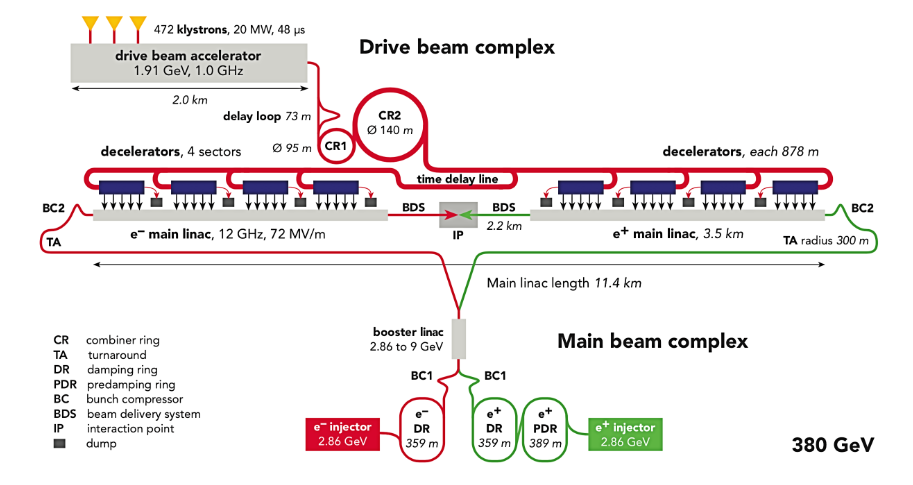
\includegraphics[width=.8\textwidth]{IMG/Cap1/CLIC.png}
	\caption{Schematic layout of the CLIC at the 380 GeV staged option \cite{CLIC_img}.}
	\label{fig:CLIC}
\end{figure}

\section{IDEA Detector concept} \label{sec:Idea_project}
IDEA (Innovative Detector for Electron-positron Accelerators) is an innovative multi-purpose detector concept, designed to study electron-positron collisions in a wide energy range as provided by high-luminosity electroweak factories.
The detector concept was proposed in 2017 and included in conceptual design reports of both FCC-ee \cite{FCC-ee_design} and CEPC \cite{CEPC_design}.

\begin{figure}
	\centering
	\subfloat[][ Artistic view of the IDEA detector concept. \label{fig:IDEA_art1}]{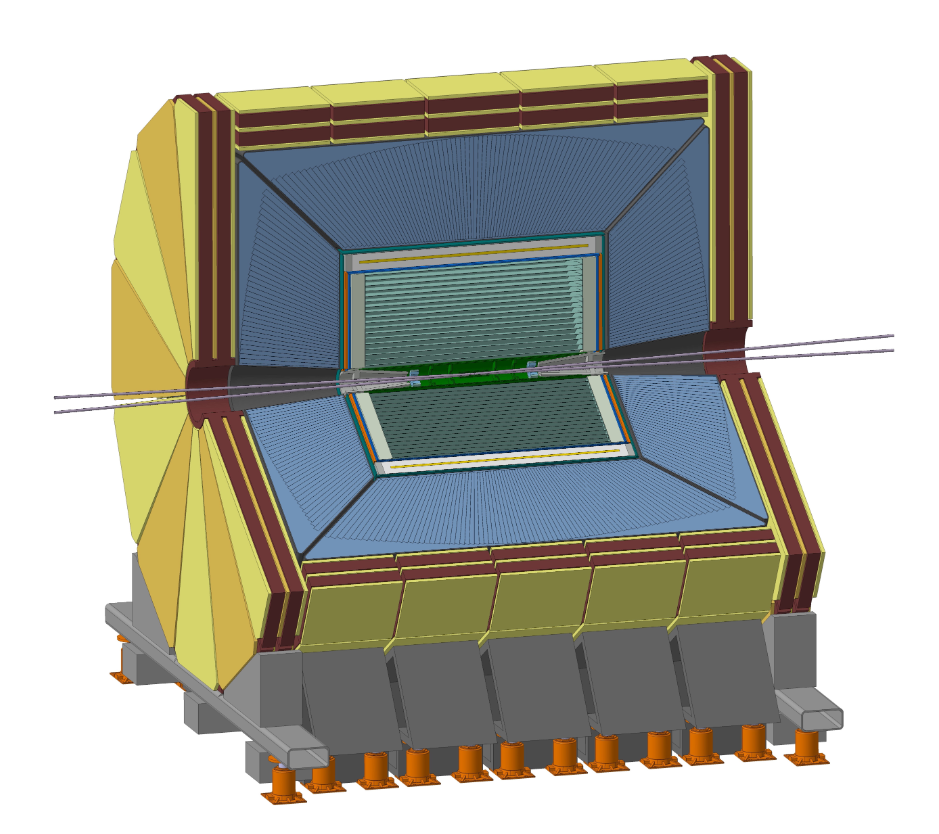
\includegraphics[width=.45\textwidth]{IMG/Cap1/IDEA_art1}} \quad
	\subfloat[][The structure and dimensions of the IDEA detector concept. \label{fig:IDEA_art2}]{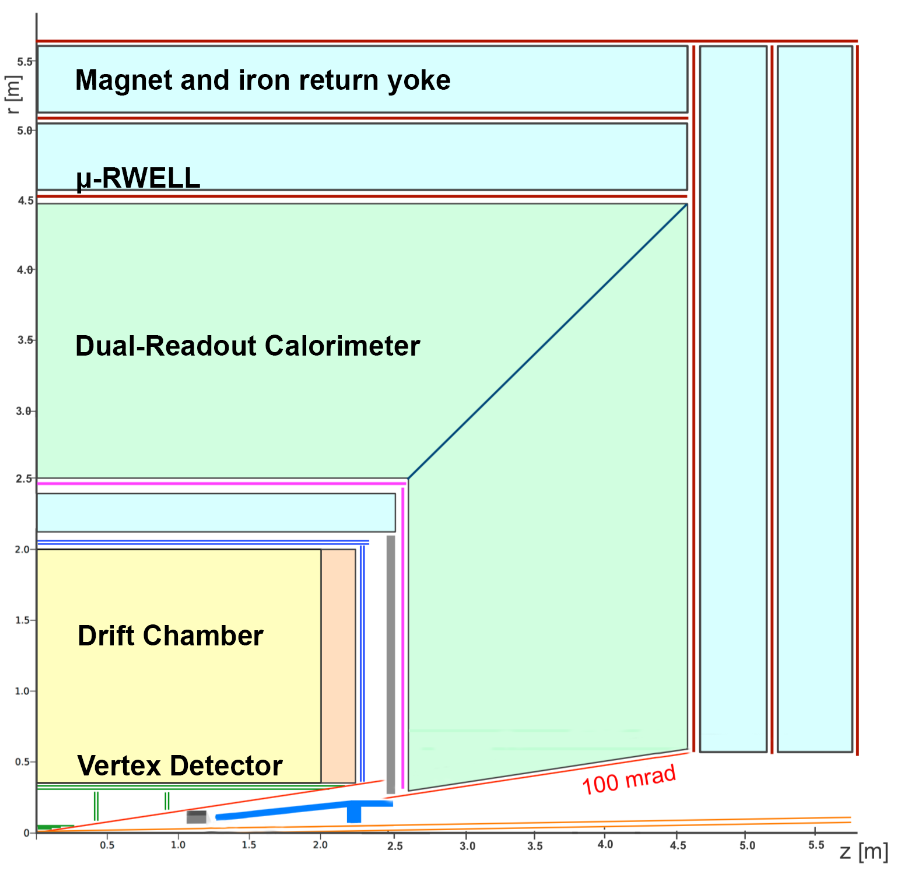
\includegraphics[width=.45\textwidth]{IMG/Cap1/IDEA_art2}}
	\caption{The IDEA detector concept.}
\end{figure}

The IDEA Detector concept is sketched in an artistic view in Figure \ref{fig:IDEA_art1} and in its structure and dimensions in Figure \ref{fig:IDEA_art2}. 
The overall detector is composed by a silicon pixel vertex detector, a wire chamber surrounded by a layer of silicon micro-strip detectors, a thin superconducting solenoid coil, a preshower detector, a dual-readout calorimeter and a muon spectrometer.
The most innovative elements proposed are:
\begin{itemize}
  \item an ultra-light drift chamber as main tracker;
  \item a Dual-Readout (DR) fibre-sampling calorimeter, for both electromagnetic and hadronic shower measurement.
\end{itemize}

The Drift CHamber (DCH) technology is based on the R\&D work done for the upgrade of the MEG experiment (MEG II), designed to search for the charged lepton flavor violating decay $\mu \rightarrow e\gamma$. This work involves the construction of an ultra-light drift chamber performing high momentum resolution and high transparency in terms of radiation length.
The IDEA dual-readout calorimeter, on the other hand, stands on the legacy of the DREAM/RD52 Collaboration. The key point is the expected performance of dual-readout optical-fibre calorimeters in obtaining high-resolution energy measurements for both single hadrons and hadronic jets.
All the most important parameters of the IDEA detector components are listed in Table \ref{tab:IDEA_part}.\\
\begin{table}
  \centering
  \begin{tabular}{ll}
    \toprule
    Vertex technology                       & Silicon \\
    Vertex inner/outer radius (cm)          & $1.7/34$ \\
    \midrule
    Tracker technology                      & Drift Chamber and Silicon Wrapper\\
    Tracker half length (m)                 & $2.0$ \\
    Tracker outer radius (m)                & $2.0$ \\
    \midrule
    Solenoid field (T)                      & $2.0$ \\
    Solenoid bore radius / half length (m)  & $2.1/30.$ \\
    \midrule
    Preshower absorber                      & Lead \\
    Preshower $R_{min}/R_{max}$ (m)         & $2.4/2.5$ \\
    \midrule
    Calorimeter absorber                    & Copper \\
    Calorimeter $R_{min}/R_{max}$ (m)       & $2.5/4.5$ \\
    \midrule
    Overall height / length (m)             & 11/13 \\
    \bottomrule
  \end{tabular}
  \caption{Parameters of the different sub-detectors composing IDEA.}
  \label{tab:IDEA_part}
\end{table}

\subsection{Vertex detector}
The $1.5$ cm beam pipe is surrounded by the IDEA vertex detector composed by pixel active sensors. The structure present a high-resistivity substrate architecture implementing on-pixel sparsification and data-driven, time-stamped readout.
The goal is a thickness of $0.15-0.30\%\ X_0$ per layer and a power dissipation below $20$ mW$/$cm$^2$.

The tracks of charged particles are measured with very high precision, of the order of $3$ $\mu$m in the innermost layers. The vertex detector must also be able to precisely reconstruct secondary vertices.
%This detector will significantly benefit from the electronic and mechanical work for the ALICE ITS \cite{alice_its}, as well as of new ongoing developments, in the framework of the INFN ARCADIA R\&D project.
%%%

\subsection{Drift chamber}
Based on the experience with the KLOE Experiment DCH \cite{KLOE} and the recent DCH for the MEG upgrade \cite{MEG2}, a similar detector, with extraordinary transparency to charged particles, has been proposed for the IDEA Experiment.\\

The chamber is composed by a unique cylindrical volume, coaxial to the beam axis, with an inner radius of $0.35$ m and an outer radius of $2$ m, for a total length of $4$ m. It consists of $112$ coaxial layers, at alternating-sign stereo angles, grouped in $24$ identical sectors. The total number of drift cells is $56448$ with variable size from $12.0$ to $14.5$ mm.
The chamber is operated with a very light gas mixture of $90\%$ He - $10\%$ iC$_4$H$_{10}$ (isobutane), providing a maximum drift time value of $\simeq 400$ ns.\\
The angular coverage extends down to $\simeq 13\deg$, and could be extended with additional silicon disks between the DCH and the calorimeter end caps.\\
In the radial direction the total amount of material is of the order of $1.6\%$ of a radiation length ($X_0$), including the inner and outer cylindrical walls and the contributions due to the gas mixture and the wires. On the other hand, in the forward and backward direction, the total amount of material is equivalent to about $5.0\%\ X_0$, including the inner cylindrical walls and the service end plates, instrumented with front-end electronics, signal and HV cables.\\

In the context of the MEG2 drift chamber prototypes \cite{MEG2} with $7$ mm cell size, a drift distance resolution of $100$ $\mu$m has been achieved with both a gas mixture and operating conditions very similar to the ones foreseen for the IDEA DCH.
Analytical calculations, in such operating conditions, were used to estimate the momentum and angular resolutions with the results shown in Figure \ref{fig:DCH_res}.
The drift chamber also offers outstanding particle-identification performance using the cluster counting technology that improves, as well, the spatial resolution.

%Together with the excellent expected momentum resolution, the DCH can achieve superior particle identification capabilities thanks to the cluster-counting technique.
The ionisation process, by means of which electrons are released, follows a Poison law, therefore, by counting the total number of ionisation clusters ($N_{cl}$) of a charged track, one can reach a relative resolution on $N_{cl}$ that scales as  $1/\sqrt{N_{cl}}$. The expected performance relative to particle separation, in terms of number of standard deviations as a function of the particle momentum, is shown in Figure \ref{fig:DCH_separation}. In this graph the solid curves refer to the cluster-counting technique, while the dashed ones refer to the expected identification power for the traditional $dE/dx$ method. As it can be seen, the particle separation by cluster counting performs better over the whole momentum range.

\begin{figure}
	\centering
	\subfloat[][Momentum and angular resolutions for $\theta= 90^{\circ}$ as a function of particle momentum. \label{fig:DCH_res}]{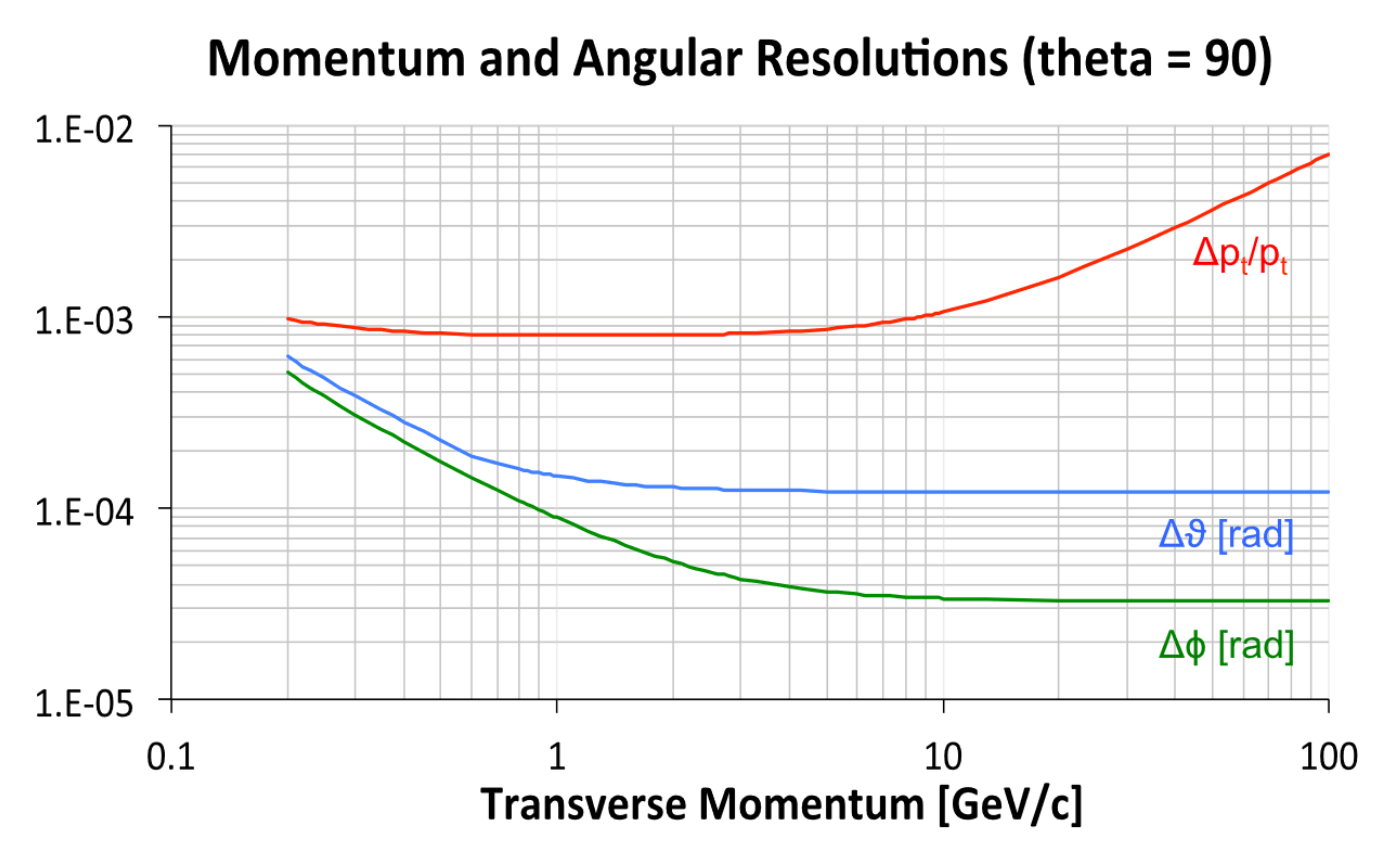
\includegraphics[width=.45\textwidth]{IMG/Cap1/DCH_res.png}} \quad
	\subfloat[][Particle-type separation in units of standard deviations as a function of momentum, with cluster counting (solid curves) and with $dE/dx$ (dashed curves). \label{fig:DCH_separation}]{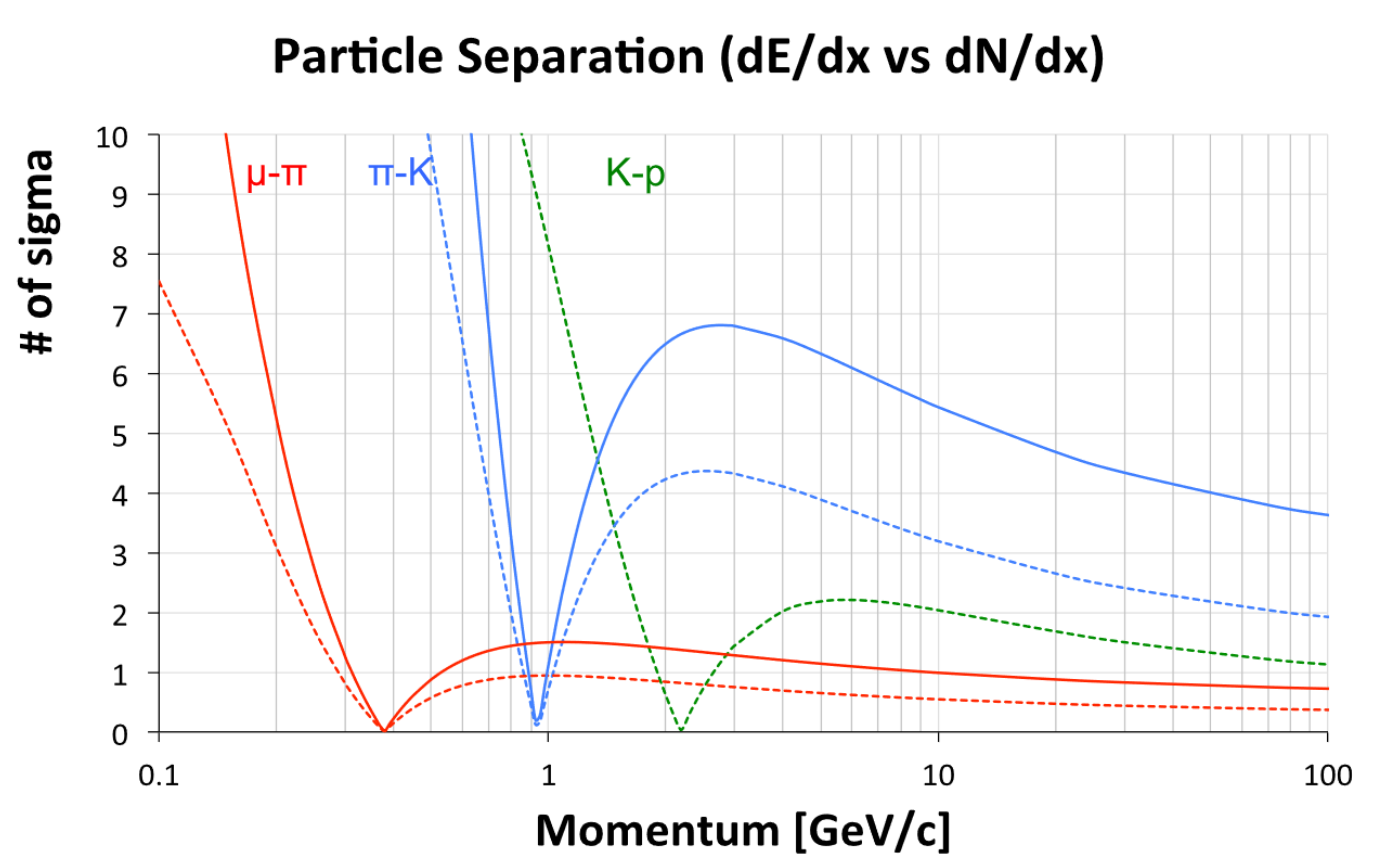
\includegraphics[width=.45\textwidth]{IMG/Cap1/DCH_separation.png}}
	\caption{IDEA ultra-light drift-chamber performance \cite{FCC-ee_design}.}
\end{figure}

\subsection{Magnet system}
The IDEA detector magnet is an ultra-thin and ultra-light (thus “radiation-transparent”) superconducting solenoid. It is $5$ m long and has an inner diameter of $4.2$ m. The main feature is that the solenoid is positioned between the tracking detectors and the calorimeter, a solution currently employed in ATLAS.
This choice requires to mantain the total thickness at the $30$ cm level, and below $1\ X_0$ in terms of radiation length, but at the same time the stored energy is reduced by a factor of four and the cost can be halved.
In this scenario a relatively low field of $2$ T can be produced.
%The flux return yoke scales with the square of the coil diameter, thus with the given dimensions a yoke thickness of less than $100$ cm of iron is sufficient to contain the magnetic flux and to shield the muon chambers.

\subsection{Dual-readout calorimeter}
The IDEA calorimeter consists of a dual-readout projective fibre-sampling detector. It follows the lessons of the high-resolution fibre calorimeters built by SPACAL \cite{SPACAL} and RD52 \cite{RD52}.\\
The detector is a tower-based, longitudinally unsegmented, fully projective calorimeter sketched in Figure \ref{fig:DRCal_geo}.
%The detector is a $4\pi$ calorimeter that does not present segmentation longitudinally, but only in the direction towards the Interaction Point (IP).
The segmentation is chosen to have the shower development confined in a small number of towers and most of the energy deposited in a single tower.
This highly simplifies the calibration procedures for which each cell response can be considered individually.
Considering that in accelerator-based experiments all the particles come, in good approximation, from the Interaction Point (IP), the projective segmentation can be obtained with a tower-based structure.\\

DR calorimeters, as described in Section \ref{sec:DRComp}, are composed by an absorber and two different active media to induce and transport two different signals. A single medium with two different response processes (such as a crystal producing both scintillation and Cherenkov light) may also be used.
In the IDEA DR calorimeter, a copper (or brass) matrix is used as absorber, filled with optical fibres as active volumes (the dual-readout method will be described in the next chapter).
The possibility to independently read out each fibre with a dedicated Silicon PhotoMultiplier (SiPM), as described in \cite{Massi_tesi}, brings a series of advantages especially in terms of spatial and angular resolution, removing the limitations arising from a readout driven by the tower dimension. For example, two particle showering in the same tower, in this way, could still be identified.\\

\begin{figure}
	\centering
	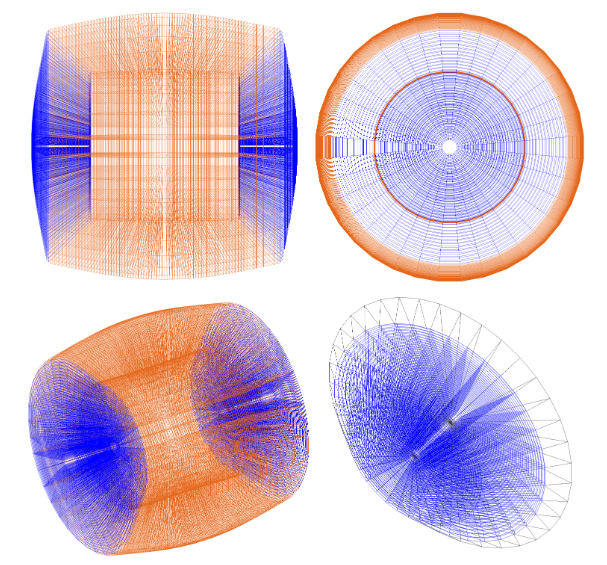
\includegraphics[width=.9\textwidth]{IMG/Cap1/DRCal_geo.png}
	\caption{IDEA dual-readout calorimetry geometry produced with GEANT4, seen from different perspectives. In orange the towers composing the barrel, in blue the ones composing the end caps.}
	\label{fig:DRCal_geo}
\end{figure}

The geometry of the calorimeter, from different perspectives, is shown in Figure \ref{fig:DRCal_geo}. Towers are truncated pyramids pointing to the IP. In such a way, each tower cover a specific region $(\Delta \theta, ~\Delta\varphi)$ of the solid angle.\\
The cylindrical symmetry is achieved through a rotation around the beam axis of a minimal structure called slice. A single slice covers a range of $10\degree$ of the $\varphi$ angle, therefore $36$ of these elements cover the full calorimeter volume.
In each slice both barrel and end-cap towers are present, in particular $80$ towers for the barrel and $35$ for each end cap, with an approximate $\theta$ coverage of $1.125\degree$ per tower.\\
All the towers are $2$ m long, composed by an absorber matrix (copper, in the actual simulation) filled with optical fibres.
The active elements are scintillating (polystyrene) and clear-plastic fibres (PolyMethyl MethAcrylate - PMMA).
The fibres are $\sim 1$ mm thick and are disposed in a chess-board like geometry so that each fibre is separated from the closest ones by $\sim 0.5$ mm of absorber material.
This complex geometry has been reproduced within the GEANT4 simulation toolkit \cite{GEANT4} and all results in this thesis are obtained with it.

\subsection{Preshower and muon chambers}
In the barrel region, just before the calorimeter, the magnet coil, coupled with Micro-Pattern Gaseous Detector (MPGD) chambers, acts as a preshower.
In the forward regions, preshower detectors are located between the drift chamber and the end-cap calorimeters.
Externally, the overall detector is surrounded by an iron return joke, to contain the magnetic field, and this volume is also instrumented with MPGD chambers, to allow muon detection and momentum measurement.
Both the preshower and the muon chambers are based on the micro-Resistive WELL ($\mu$-RWELL) technology. $\mu$-RWELL chambers are compact MPGD detectors, with a single, intrinsically spark protected, amplification stage. \\
The evaluation of the preshower performance and the single-hit-position resolution requirement are still in progress.
However, experimental results with small prototypes already show a good acceptance for photons and an efficiency of $\simeq 30\%$ for tagging $\pi^0$ from their $\gamma\gamma$ decay.\\
Also the requirements for the muon system look to be within reach. Indeed, this technology provides good tracking efficiency, high-voltage stability, a position resolution of $200-300$ $\mu$m and a good time resolution, thanks to the fast charge amplification process.\\
%Also the muon detector uses as well the $\mu$-RWELL technology but with a wider strip pitch, due to the greater dimensions. It is subdivided in three active layers at increasing distance from the vertex, and located within the iron return yoke that closes the magnetic field. Each MPGD can provide a space point with a spatial resolution of about $400$ $\mu$m in the plane perpendicular to the particle direction. Combining the three stations allows to perform standalone tracking of charged particles at $5-6$ m from the vertex. Such a precision also allows to identify secondary vertices that could be produced by long lived particles.
